% Compile with XeLaTeX (twice) or Tectonic. Unicode fonts preserve team names.
\documentclass[a4paper,11pt,oneside]{book}
\usepackage{fontspec}
\IfFontExistsTF{Times New Roman}{\setmainfont{Times New Roman}}{\setmainfont{TeX Gyre Termes}}
\IfFontExistsTF{Arial}{\setsansfont{Arial}}{\setsansfont{TeX Gyre Heros}}
\usepackage[english]{babel}
\usepackage[margin=25mm,headheight=14pt]{geometry}
\usepackage{graphicx}
\usepackage{array,longtable,booktabs,tabularx}
\usepackage{enumitem}
\usepackage{xcolor}
\usepackage{tikz}
\usetikzlibrary{arrows.meta,positioning,shapes.geometric}
\usepackage{microtype}
\usepackage[unicode,hidelinks]{hyperref}
\hypersetup{pdftitle={AI-powered Film Photography Platform: Software Engineering Report},pdfauthor={CNPM Project Team}}
\setcounter{secnumdepth}{2}
\setcounter{tocdepth}{1}
\setlength{\parindent}{0pt}
\setlength{\parskip}{6pt}
\setlength{\emergencystretch}{3em}
\setlist{itemsep=3pt,topsep=5pt}
\renewcommand{\arraystretch}{1.15}

\begin{document}
\hypersetup{pageanchor=false}
\begin{titlepage}
\centering
{\Large SOFTWARE ENGINEERING PROJECT\par}
\vspace{12mm}
{\Huge\bfseries AI-powered Platform\par}
\vspace{4mm}
{\LARGE Connecting Film Photography Enthusiasts\par}
\vspace{2mm}
{\LARGE with Film Processing Labs\par}
\vspace{12mm}
{\large Proposal, System Design, and Prototype Handover\par}
\vspace{15mm}
\begin{tabular}{ll}
\toprule
\textbf{Team member} & \textbf{Primary work package}\\
\midrule
Nguyễn Thái Gia Bảo & Context and business requirements\\
Lê Thị Như Quân & Architecture and database\\
Huỳnh Gia Hợp & Backend and API\\
Nguyễn Đào Quốc Khánh & Mobile and web applications\\
Nguyễn Thành Toàn & AI, testing, and deployment\\
\bottomrule
\end{tabular}
\vfill
{\large Submission snapshot: 17 September 2026\par}
\vspace{5mm}
\url{https://github.com/thanhtoan101/CNPM}
\end{titlepage}

\frontmatter
\hypersetup{pageanchor=true}
\chapter*{Report Scope}
\addcontentsline{toc}{chapter}{Report Scope}
This report consolidates the team's proposal, requirements, architecture, and
mobile/web design. Statements using ``shall'', ``will'', and ``proposed'' define
the intended platform and its acceptance criteria; they do not imply that every
feature has already been implemented or deployed.

The repository contains a React/TypeScript web prototype, a Flutter mobile
prototype, an Express backend, and a separate Python AI prototype. The frontend
demonstration uses local data. A working user interface does not establish
successful payment, real cloud scan delivery, cross-device synchronization,
or production authentication. The final chapter records the implementation
boundaries and a reproducible demonstration checklist.

Task ownership describes agreed responsibilities. Git history and Jira work
items provide change evidence; a planned allocation of 20\% per member is not
a measured contribution percentage. Evaluation must consider the content,
tests, and documented work as well as commit counts.

{\small\tableofcontents}
\listoffigures
\listoftables
\mainmatter
\chapter{Project Proposal and Requirements}
% ==========================================
% 3.2.a CONTEXT
% Responsible member: Bao
% ==========================================

\section*{3.2.a Context}
\addcontentsline{toc}{section}{3.2.a Context}

\subsection{Background}

In recent years, film photography has experienced a significant revival worldwide, including in Vietnam. Increasing numbers of photography enthusiasts, artists, and collectors are returning to analog photography because of its distinctive aesthetic qualities, creative experience, and the tangible value of physical film. Unlike digital photography, film photography requires a more deliberate shooting process and produces unique visual characteristics that cannot always be replicated by digital filters.

As the analog photography community continues to grow, the demand for supporting services such as film developing, film scanning, photo printing, film preservation, and digital archiving has also increased. However, the service ecosystem surrounding film photography remains highly fragmented. Photographers often need to search for Film Labs through social media platforms, online communities, messaging applications, or personal recommendations. Information regarding service availability, pricing, turnaround time, supported film formats, processing quality, and customer reviews is usually distributed across multiple channels.

\subsection{Current Problems}

Currently, there is no centralized digital platform that allows photographers to conveniently search, compare, book, and monitor film processing services. Customers usually communicate with Film Labs manually through social media, messaging applications, or phone calls to inquire about available services and order status. This communication process can be time-consuming and may lead to inconsistent information, delayed responses, and difficulties in tracking orders.

From the perspective of Film Labs, many laboratories still rely on manual workflows for receiving film rolls, recording customer information, monitoring processing stages, delivering digital scan files, and managing business operations. These fragmented processes may reduce operational efficiency and make it more difficult for Film Labs to scale their services as customer demand increases.

In addition, the analog photography community lacks an integrated digital ecosystem that combines professional services with community interaction. Photographers need not only reliable Film Lab services but also access to photography knowledge, equipment reviews, community discussions, workshops, photowalk events, and opportunities to buy or sell analog photography equipment. Digital scan files are also often stored separately across different cloud storage services, making it difficult for photographers to maintain a structured and searchable personal film archive.

\subsection{Project Motivation}

The growing popularity of film photography and the fragmented nature of the current service ecosystem create an opportunity for digital transformation. A centralized platform can improve the connection between photographers and Film Labs by providing transparent service information, standardized booking processes, real-time order tracking, and digital delivery of scanned photographs.

At the same time, the rapid development of Artificial Intelligence provides additional opportunities to improve the user experience. AI technologies can be applied to recommend suitable Film Labs based on user preferences, assist photographers in selecting appropriate film types, analyze scan quality, support intelligent search, and provide photography-related guidance through a domain-specific conversational assistant.

Therefore, this project proposes the development of an AI-powered digital platform that connects photographers, Film Labs, photography experts, delivery partners, and administrators within a unified ecosystem. The platform aims to digitalize film processing services, improve operational efficiency for Film Labs, facilitate knowledge sharing and community engagement, and provide intelligent and personalized services for analog photography enthusiasts.

\subsection{Project Objective and Significance}

The main objective of the project is to establish a scalable digital ecosystem that supports the complete lifecycle of analog photography. The proposed platform will allow photographers to discover Film Labs, compare available services, place service orders, request pickup and delivery, monitor processing progress, receive digital scans, and manage photographs through a personal Digital Film Archive.

For Film Labs, the platform will provide digital tools for service management, workflow monitoring, customer management, digital file delivery, and business analytics. Photography experts will be able to contribute tutorials, technical articles, equipment reviews, and professional knowledge to the community. Delivery partners can participate in the logistics process for film collection and delivery, while system administrators can monitor platform operations and ensure a reliable environment for all stakeholders.

By integrating Artificial Intelligence, cloud storage, digital asset management, and community-based services, the project is expected to modernize the analog photography ecosystem and create a sustainable platform that benefits both photographers and service providers.


% ==========================================
% 3.2.b PROPOSED SOLUTIONS
% Responsible member: Hop
% ==========================================

\section*{3.2.b Proposed Solutions}
\addcontentsline{toc}{section}{3.2.b Proposed Solutions}

% Hop: Write the Proposed Solutions section here.

% ==========================================
% 3.2.c FUNCTIONAL REQUIREMENTS
% Responsible member: Khanh
% ==========================================

\section*{3.2.c Functional Requirements}
\addcontentsline{toc}{section}{3.2.c Functional Requirements}

% Khanh: Write the Functional Requirements section here.

\section{Use Case Specification and Business Rules}
The six use cases refine the business flows into reviewable contracts. They
describe the target platform. A success condition in this section is an
acceptance requirement, not evidence that the integration already exists.
The identifiers UC-01--UC-06 are local report identifiers and do not create
additional Jira tasks.

\subsection{Use Case Overview}
\begin{figure}[htbp]\centering
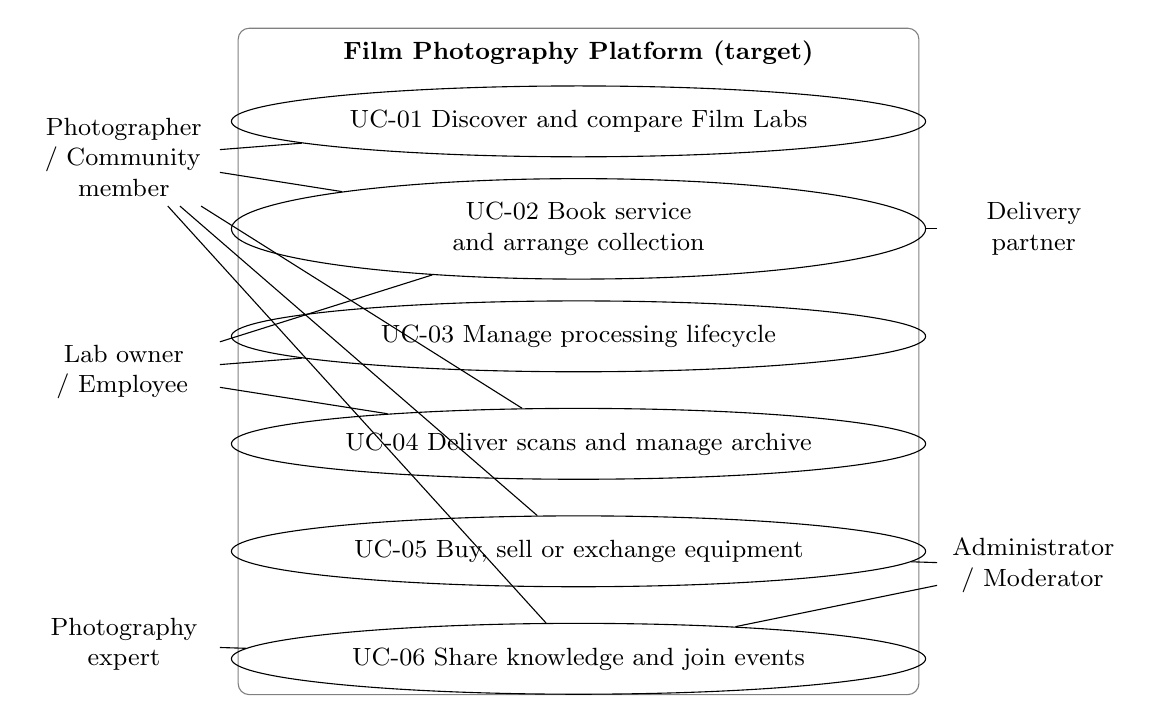
\begin{tikzpicture}[x=0.91cm,y=0.91cm,font=\small,
 uc/.style={draw,ellipse,text width=6cm,align=center,minimum height=9mm},
 actor/.style={align=center,text width=2.2cm}]
\draw[rounded corners,gray] (2.5,0.8) rectangle (12,-8.5);
\node[font=\small\bfseries] at (7.25,0.45) {Film Photography Platform (target)};
\node[uc] (u1) at (7.25,-0.5) {UC-01 Discover and compare Film Labs};
\node[uc] (u2) at (7.25,-2) {UC-02 Book service and arrange collection};
\node[uc] (u3) at (7.25,-3.5) {UC-03 Manage processing lifecycle};
\node[uc] (u4) at (7.25,-5) {UC-04 Deliver scans and manage archive};
\node[uc] (u5) at (7.25,-6.5) {UC-05 Buy, sell or exchange equipment};
\node[uc] (u6) at (7.25,-8) {UC-06 Share knowledge and join events};
\node[actor] (p) at (0.9,-1) {Photographer / Community member};
\node[actor] (l) at (0.9,-4) {Lab owner / Employee};
\node[actor] (e) at (0.9,-7.8) {Photography expert};
\node[actor] (d) at (13.6,-2) {Delivery partner};
\node[actor] (m) at (13.6,-6.7) {Administrator / Moderator};
\draw (p)--(u1);\draw (p)--(u2);\draw (p)--(u4);\draw (p)--(u5);\draw (p)--(u6);
\draw (l)--(u2);\draw (l)--(u3);\draw (l)--(u4);
\draw (d)--(u2);\draw (m)--(u5);\draw (m)--(u6);\draw (e)--(u6);
\end{tikzpicture}
\caption{Business use case associations; supporting AI and storage services are shown in the architecture}
\end{figure}

\clearpage
\subsection{UC-01: Discover and Compare Film Labs}
\textbf{Primary actor:} Photographer. \textbf{Trigger:} open discovery or submit filters.
\textbf{Preconditions:} a searchable lab catalogue exists; personalization is
optional. \textbf{Success:} the selected lab and service remain available for
the booking preview. \textbf{Failure guarantee:} searching does not create an order.
\begin{enumerate}
\item Enter location, film format, budget or turnaround preferences.
\item Validate filters and retrieve matching active lab services.
\item Rank eligible results; optional AI recommendations explain their basis.
\item Inspect price, supported formats, address and estimated turnaround.
\item Select a lab and continue with its current service catalogue.
\end{enumerate}
\textbf{Exceptions:} no matches preserves filters and suggests changing them;
missing history uses ordinary ranking; unavailable AI leaves normal search
available. A removed service must be revalidated before booking.
\textbf{Acceptance:} a keyword and film-format filter apply together; zero results
show an explicit empty state; choosing a result opens the correct lab.
\textbf{Trace:} US-01, SCRUM-5/28, \path{apps/mobile/lib/screens/home_screen.dart}.
Mobile filtering uses sample data; AI ranking is a separate Python module.

\subsection{UC-02: Book Service and Arrange Collection}
\textbf{Primary actor:} Photographer. \textbf{Supporting actors:} Lab and delivery
partner. \textbf{Preconditions:} signed-in customer, active service at the selected
lab, positive integer quantity. \textbf{Success:} an order ID, price snapshot and
collection choice are recorded. \textbf{Failure guarantee:} invalid inputs do not
create an order or charge the customer.
\begin{enumerate}
\item Select service, film details, scan options and quantity.
\item Choose direct drop-off or supply pickup address and time.
\item Calculate the estimate and show service and collection charges separately.
\item Confirm; the API checks ownership, availability and authoritative price.
\item Persist the order and request collection if required.
\item Display order code; the lab accepts or rejects capacity-dependent work.
\end{enumerate}
\textbf{Exceptions:} unavailable service requires reselection; unavailable pickup
offers another slot/drop-off; missing fields remain editable; a repeated request
must not create duplicate orders in the target integration.
\textbf{Acceptance:} quantity zero, fractional or above 100 is rejected by the
current API; a client-supplied total cannot override the catalogue price.
\textbf{Trace:} US-02, BR-02, SCRUM-6/28. Mobile is a preview; the independent
API implements basic creation without pickup, payment or idempotency.

\clearpage
\subsection{UC-03: Manage the Processing Lifecycle}
\textbf{Primary actor:} Lab employee. \textbf{Preconditions:} authenticated staff
assigned to the order's lab; received film matches the request.
\textbf{Success:} a permitted stage change records actor, time and notes.
\textbf{Failure guarantee:} an invalid transition does not alter the last valid state.
\begin{enumerate}
\item Find the order and inspect requested service, rolls and handling notes.
\item Verify the physical receipt and record discrepancies before processing.
\item Advance through development, washing/drying, scanning and preparation.
\item Inspect quality; record a rework or delay when needed.
\item Save the stage history and notify the customer of relevant changes.
\end{enumerate}
\textbf{Exceptions:} damaged film pauses the target workflow; failed quality
requires a recorded rework; a stale concurrent update must be rejected rather
than overwrite a newer stage. Offline retention and resynchronization are target
requirements, not current web behavior.
\textbf{Acceptance:} only a permitted next stage is offered; completed orders
cannot advance; a scan order at quality check cannot complete without reviewed
publication. \textbf{Trace:} US-03/04, BR-03, SCRUM-8/29, web domain tests.
The demo combines physical substeps and persists browser state only.

\subsection{UC-04: Deliver Scans and Manage the Archive}
\textbf{Primary actor:} Lab employee, followed by photographer.
\textbf{Preconditions:} scan order at quality check, files ready for review and
authorized customer ownership. \textbf{Success:} reviewed scans are available
privately to the correct customer. \textbf{Failure guarantee:} rejected files
are not published; pending transfers do not mark delivery complete.
\begin{enumerate}
\item Select the order and scan files; validate type, size and duplicate names.
\item Transfer bytes to private storage and verify successful transfer.
\item Review image quality and available film/camera/scan metadata.
\item Confirm publication; save metadata and append a release audit record.
\item Notify the customer, who can view, download, tag and organize the images.
\end{enumerate}
\textbf{Exceptions:} invalid/corrupt files require replacement; transfer failures
remain pending; unauthorized reads are denied; optional missing metadata can be
added later without changing the original scan bytes.
\textbf{Acceptance:} the local prototype accepts 1--100 JPEG/TIFF files,
each greater than zero and at most 50 MiB; review and release confirmations are
required; duplicate publication is rejected. Filename/MIME validation is not
file-content inspection. \textbf{Trace:} US-05/06, BR-04/05, SCRUM-9/29/31.
Only private metadata is saved locally; cloud transfer/download remains planned.

\clearpage
\subsection{UC-05: Buy, Sell or Exchange Equipment}
\textbf{Primary actors:} Seller and buyer. \textbf{Supporting actor:} Moderator.
\textbf{Preconditions:} signed-in users and a valid active listing.
\textbf{Success:} a transaction and final listing state are recorded.
\textbf{Failure guarantee:} an unavailable listing cannot open a new transaction.
\begin{enumerate}
\item Seller enters category, condition, description, price and photographs.
\item Validate and publish the listing; buyers search and inspect its details.
\item Buyer contacts the seller and requests purchase or exchange.
\item Seller confirms; the system records reservation and transaction status.
\item Record fulfillment or cancellation, then allow eligible feedback.
\end{enumerate}
\textbf{Exceptions:} incomplete listings stay draft; sold/hidden/expired items
reject requests; disputes preserve evidence and reach the moderation queue;
simultaneous buyers require server-side reservation consistency.
\textbf{Acceptance:} visibility and availability have explicit labels; a moderation
decision requires a reason, updates the linked listing when applicable and
records an audit event. \textbf{Trace:} US-07/08, BR-06/07, SCRUM-10/30/31.
The prototype supports catalogue and local moderation; payment, messaging,
reservation and transaction fulfillment are not implemented end to end.

\subsection{UC-06: Share Knowledge and Join Events}
\textbf{Primary actors:} Expert and community member. \textbf{Supporting actor:}
Moderator. \textbf{Preconditions:} contributor is permitted to publish; event
dates and capacity are valid. \textbf{Success:} content or registration is stored
and visible to the appropriate audience. \textbf{Failure guarantee:} rejected
content is not silently published; a full event does not overbook.
\begin{enumerate}
\item Author submits an article, tutorial, review or event description.
\item Validate required content and perform the applicable moderation review.
\item Publish accepted content so members can search, read and discuss it.
\item Register interested members while checking capacity and duplicate entries.
\item Send event changes/reminders and preserve useful follow-up discussion.
\end{enumerate}
\textbf{Exceptions:} reported content enters review; full events close or waitlist;
cancellation notifies registrants; duplicate registration returns the existing
registration rather than consuming another seat.
\textbf{Acceptance:} date range is valid, moderation is traceable and capacity
cannot be exceeded under concurrent registration.
\textbf{Trace:} Core Flow 6, BR-08, SCRUM-10. The backend has basic course
creation/date validation; article, discussion, enrollment and notification
services remain target work.

\subsection{Shared Business Rules}
\begin{longtable}{p{0.13\textwidth}p{0.78\textwidth}}
\toprule\textbf{Rule} & \textbf{Required invariant}\\\midrule\endhead
BR-01 & Access is scoped by role and resource ownership; a portal switch is not authentication.\\
BR-02 & Booking quantity is a positive integer; server catalogue determines the persisted price.\\
BR-03 & Processing follows permitted transitions; the history retains actor, time and exception notes.\\
BR-04 & Scans belong to the selected order/customer and require quality review before release.\\
BR-05 & New delivery is private; personal organization does not overwrite original scan files.\\
BR-06 & Unavailable marketplace listings cannot accept new transactions.\\
BR-07 & Administrative decisions require evidence, appropriate reasons and an audit record.\\
BR-08 & Events respect capacity; changes and cancellation reach registered members.\\
BR-09 & AI discloses insufficient evidence; ordinary search remains available independently.\\
BR-10 & Demo data and proposed targets are never presented as measured production results.\\
\bottomrule
\end{longtable}

% ==========================================
% 3.4 TECHNICAL REQUIREMENTS
% Responsible member: Quan
% ==========================================

\section{Technical Requirements}

This section defines the non-functional and technical requirements of the
AI-powered Film Photography Platform. These requirements focus on security,
performance, reliability, scalability, maintainability, data consistency,
and system integration to ensure that the proposed platform can operate
effectively for photographers, Film Labs, photography experts, delivery
partners, administrators, and AI services.

\subsection{Security and Access Control}

The platform shall provide secure authentication and authorization mechanisms
for all users and system components.

\begin{itemize}
    \item The system shall support secure user authentication using JSON Web
    Token (JWT) and may support OAuth2-based external identity integration.

    \item Role-Based Access Control (RBAC) shall be used to manage permissions
    for different roles, including Photographer, Film Lab Owner,
    Photography Expert, Delivery Partner, System Administrator, and
    AI Assistant.

    \item Users shall only be allowed to access functions and information
    permitted by their assigned roles.

    \item Passwords and other sensitive credentials shall not be stored
    in plain text.

    \item Personal information, order information, payment-related information,
    and digital film scan files shall be protected against unauthorized access.

    \item Communication between client applications, backend services,
    and external APIs shall use secure communication protocols such as HTTPS.
\end{itemize}

\subsection{Data Storage and Protection}

The system shall provide reliable and consistent storage for both structured
business data and digital media files.

\begin{itemize}
    \item PostgreSQL shall be used to store structured data such as user
    accounts, Film Lab profiles, services, orders, reviews, and other
    system information.

    \item Digital film scans and other large media files shall be stored using
    cloud storage such as Azure Blob Storage or Firebase Storage.

    \item The system shall provide backup and recovery mechanisms to reduce
    the risk of data loss.

    \item Access to stored digital scans shall be controlled according to
    user permissions and ownership of the corresponding orders or resources.

    \item Data shall remain consistent when multiple users or services
    access and modify the system simultaneously.
\end{itemize}

\subsection{Performance}

The platform shall provide responsive services for common user and Film Lab
operations under normal operating conditions.

\begin{itemize}
    \item Common operations such as searching Film Labs, viewing services,
    checking order status, and accessing user information shall provide
    responsive results under normal operating conditions.

    \item Database queries shall be designed efficiently to support frequent
    searches, transactions, and order-related operations.

    \item The system shall support efficient upload, storage, and retrieval
    of digital film scan files.

    \item Caching and search optimization may be applied to improve response
    time for frequently requested information.
\end{itemize}

\subsection{Availability and Reliability}

The system shall remain reliable during normal operation and shall minimize
service interruptions.

\begin{itemize}
    \item The platform shall provide high availability for core services
    used by photographers and Film Labs.

    \item The system shall handle failures of individual services without
    unnecessarily affecting unrelated functions.

    \item Backup and recovery procedures shall be available for important
    application and database data.

    \item Order and processing information shall be stored consistently so
    that users can accurately track the status of their film orders.
\end{itemize}

\subsection{Scalability}

The architecture shall support future growth of the platform.

\begin{itemize}
    \item The system shall be able to accommodate an increasing number of
    photographers, Film Labs, orders, digital images, and community activities.

    \item Multiple Film Labs shall be able to operate simultaneously on
    the same platform.

    \item Backend services shall be designed so that computing resources
    can be increased when system traffic grows.

    \item Cloud infrastructure shall support future expansion of storage,
    processing, and application services.
\end{itemize}

\subsection{Modularity and Maintainability}

The platform shall use a modular architecture to simplify development,
testing, maintenance, and future upgrades.

\begin{itemize}
    \item Major components shall be separated into Mobile Application,
    Web Portal, Backend Services, AI Services, Database, Search Engine,
    and Cloud Storage.

    \item Components shall communicate through well-defined APIs and
    data interfaces.

    \item Changes to one component shall have minimal impact on
    unrelated components.

    \item AI services and other external integrations shall be designed
    so that they can be replaced or upgraded without requiring a complete
    redesign of the platform.
\end{itemize}

\subsection{API and System Integration}

The platform shall provide integration capabilities for internal and
external services.

\begin{itemize}
    \item RESTful APIs shall be used for communication between the mobile
    application, web portal, backend services, and other system components.

    \item APIs shall support integration with payment gateways, logistics
    providers, cloud storage services, and AI services.

    \item Data exchanged through APIs shall follow consistent data formats
    and secure communication mechanisms.

    \item The architecture shall allow additional photography-related
    services to be integrated in the future.
\end{itemize}

\subsection{Search and Data Access}

The platform shall provide efficient access to Film Lab and
photography-related information.

\begin{itemize}
    \item A search engine such as Elasticsearch or OpenSearch may be used
    for Film Lab, service, marketplace, and photography knowledge searches.

    \item Search results should be relevant, responsive, and filterable
    according to available system attributes.

    \item Authorized users shall be able to retrieve their own orders,
    digital scans, and related information efficiently.
\end{itemize}

\subsection{Deployment and Continuous Integration}

The system shall support modern cloud deployment and software development
practices.

\begin{itemize}
    \item Microsoft Azure may be used as the main cloud deployment platform.

    \item GitHub shall be used for source-code version control and
    team collaboration.

    \item GitHub Actions may be used to automate build, testing, and
    continuous integration and deployment (CI/CD) activities.

    \item Deployment configurations shall be separated from application
    source code where appropriate to improve security and maintainability.
\end{itemize}

% ==========================================
% 3.2.e THEORY AND PRACTICAL
% Responsible member: Quan
% ==========================================

\section*{3.2.e Theory and Practical}
\addcontentsline{toc}{section}{3.2.e Theory and Practical}

% Quan: Write the Theory and Practical section here.

% ==========================================
% 3.2.f EXPECTED DELIVERABLES
% ==========================================

\section*{3.2.f Expected Deliverables}
\addcontentsline{toc}{section}{3.2.f Expected Deliverables}

The project is expected to deliver a cloud-deployable Minimum Viable Product
(MVP) that demonstrates the complete analog photography service lifecycle,
from Film Lab discovery and service booking to processing tracking, digital
delivery, long-term archiving, and community engagement. The expected products
are described below.

\subsection*{Mobile Application for Photographers}

A cross-platform Flutter application for Android and iOS will provide the main
customer-facing experience. Photographers will be able to register and manage
their accounts, discover and compare Film Labs, configure and book services,
request pickup and delivery, complete online payments, track order progress,
receive notifications, access digital scans, manage their personal archive,
participate in community features and the Marketplace, and interact with the
AI-powered Photography Assistant.

\subsection*{Film Lab Management Web Portal}

A ReactJS or Next.js portal will allow Film Lab owners and operators to manage
laboratory profiles, supported film formats, service packages, prices,
processing capacity, and expected turnaround times. It will also support order
verification, workflow scheduling, processing-stage updates, digital scan
delivery, customer management, revenue monitoring, and operational reporting.

\subsection*{Web Administration System}

A centralized administration application will support the management of users,
roles, permissions, Film Lab approvals, service categories, transaction fees,
payments, Marketplace operations, reviews, community content, complaints, and
disputes. Audit information and platform-level monitoring will help
administrators maintain safe and consistent operations.

\subsection*{Marketplace Module}

The Marketplace will allow community members to publish, search for, buy, sell,
or exchange analog cameras, lenses, film rolls, and photography accessories.
Its scope will include listing management, search and filtering, seller
profiles, ratings, transaction tracking, and communication between buyers and
sellers.

\subsection*{Community and Knowledge-Sharing Platform}

Photography Experts and experienced community members will be able to publish
tutorials, technical articles, equipment reviews, Film Lab reviews, and
practical experiences. The platform will also support discussions, questions
and answers, workshops, photowalks, and event registration, thereby creating a
continuously expanding photography knowledge base.

\subsection*{Digital Film Archive Management System}

A secure cloud-based Digital Film Archive will allow photographers to preview,
download, classify, search, and organize scanned photographs. Each digital asset
may retain metadata such as film stock, camera model, lens, shooting date, Film
Lab, processing method, and scanning specifications. Access control, storage
policies, backup, and recovery mechanisms will protect users' collections.

\subsection*{AI Recommendation Engine}

The Recommendation Engine will use user preferences, service history,
geographical constraints, Film Lab capabilities, prices, turnaround times, and
community feedback to rank suitable Film Labs and services. It will also
support personalized film-stock and educational-resource suggestions. The
deliverable will include a callable AI service, a documented evaluation method,
and comparative results for the selected recommendation approach.

\subsection*{AI-Powered Photography Assistant}

The Photography Assistant will combine a Large Language Model with
Retrieval-Augmented Generation and a curated domain knowledge base to answer
photography-related questions with relevant context. The AI package will also
include semantic retrieval for knowledge and service discovery and a Computer
Vision prototype for detecting common scan-quality problems such as blur,
exposure errors, color casts, dust, and scratches. Evaluation results,
limitations, and responsible-use guidance will accompany these components.

\subsection*{Backend Services and Cloud Infrastructure}

A modular backend will provide RESTful APIs, PostgreSQL persistence, JWT and
OAuth2 authentication, Role-Based Access Control, multi-tenant data isolation,
cloud file storage, search indexing, and AI-service orchestration. Integration
interfaces will support payment gateways and third-party logistics providers.
The cloud infrastructure will include CI/CD, logging, monitoring, backup, and
recovery mechanisms required to deploy and operate the MVP.

\subsection*{Delivery Evidence}

The final handover will include source code, database migrations, API
specifications, architecture and database diagrams, test plans and results, AI
experiment reports, deployment instructions, user guides, technical
documentation, the final Capstone report, presentation slides, and a product
demonstration. These artifacts will provide verifiable evidence that the
products above satisfy the agreed functional and non-functional requirements.

% ==========================================
% 3.2.g CÁC NHIỆM VỤ ĐỀ XUẤT
% ==========================================

\section*{3.2.g Các nhiệm vụ đề xuất}
\addcontentsline{toc}{section}{3.2.g Các nhiệm vụ đề xuất}

To distribute the workload fairly, the project is organized into five
comparable work packages. Each member owns the analysis and design activities,
implementation or research, testing, and documentation associated with the
assigned package. The planned team capacity is allocated at approximately
20\% per member and will be monitored through sprint backlog items and story
points.

\subsection*{Gói công việc 1: Bối cảnh, giải pháp và yêu cầu nghiệp vụ}

\textbf{Người phụ trách: Nguyễn Thái Gia Bảo}

\begin{itemize}
	\item Analyze the project context, current problems, stakeholder needs, and
	the proposed value of the unified film-photography ecosystem.
	\item Define system actors, functional requirements, business rules, shared
	terminology, acceptance criteria, and the six core business flows.
	\item Prepare user stories and trace them to the relevant actors, use cases,
	and business processes.
	\item Produce the Use Case, Business Flow, and Activity diagrams and document
	the assumptions and boundaries used by the remaining work packages.
\end{itemize}

The expected outputs are the context and problem analysis, proposed solution,
actor catalogue, requirements baseline, business rules, user stories, Use Case
Diagram, and six documented Business Flows.

\subsection*{Gói công việc 2: Yêu cầu phi chức năng, cơ sở dữ liệu và kiến trúc}

\textbf{Người phụ trách: Lê Thị Như Quân}

\begin{itemize}
	\item Define measurable non-functional requirements for security,
	performance, availability, scalability, data consistency, maintainability,
	backup, and recovery.
	\item Select and justify the technology stack and design the modular,
	multi-tenant system architecture and storage architecture.
	\item Design the PostgreSQL schema, entity relationships, constraints,
	indexes, data-isolation rules, models, and migration or SQL scripts.
	\item Produce the System Architecture, Entity--Relationship, Database
	Architecture, and Storage Architecture diagrams and verify their consistency.
\end{itemize}

The expected outputs are the non-functional requirements, technology rationale,
system and storage architecture, ERD, database schema, models, migrations or SQL
scripts, and supporting architecture documentation.

\subsection*{Gói công việc 3: Hệ thống phía máy chủ và API}

\textbf{Người phụ trách: Huỳnh Gia Hợp}

\begin{itemize}
	\item Define RESTful API contracts and implement the backend with ASP.NET Core
	or Node.js, including validation, error handling, logging, and persistence.
	\item Implement JWT/OAuth2 authentication, Role-Based Access Control, user
	and authorization flows, and tenant-aware business services.
	\item Implement order and Film Lab management, processing lifecycle, payment,
	digital delivery, archive metadata, and required integration contracts.
	\item Produce the API Architecture, Sequence, and API Flow diagrams together
	with API documentation, unit tests, and backend integration tests.
\end{itemize}

The expected outputs are the backend services, documented REST API, authentication
and authorization, core business logic, payment/order/Lab management, API
diagrams, and backend test evidence.

\subsection*{Gói công việc 4: Ứng dụng di động và cổng thông tin web}

\textbf{Người phụ trách: Nguyễn Đào Quốc Khánh}

\begin{itemize}
	\item Design the UI/UX and implement the Flutter photographer application and
	responsive ReactJS or Next.js web portals.
	\item Implement the Photographer App flows, Film Lab management portal,
	System Administrator portal, Marketplace UI, and Digital Archive UI.
	\item Integrate screens with the documented backend APIs and handle loading,
	empty, validation, authorization, offline, and error states consistently.
	\item Produce the UI Flow, Component/Frontend Architecture, and relevant
	Sequence diagrams; perform usability and frontend integration tests.
\end{itemize}

The expected outputs are the Flutter application, ReactJS/Next.js web portals,
reusable UI components, responsive interfaces, UI and frontend diagrams, API
integrations, user-flow documentation, and frontend test evidence.

\subsection*{Gói công việc 5: AI, kiểm thử và triển khai}

\textbf{Người phụ trách: Nguyễn Thành Toàn}

\begin{itemize}
	\item Prepare datasets, a curated photography knowledge base, baselines, and
	evaluation protocols for Film Lab recommendation, RAG, semantic search, the
	AI Assistant, and Computer Vision-based scan-quality analysis.
	\item Implement documented AI services for recommendation, retrieval and
	grounded assistance, and detection of blur, exposure problems, color casts,
	dust, and scratches; report limitations and responsible-use considerations.
	\item Define and execute unit, contract, integration, end-to-end, security,
	performance, recovery, and AI evaluation tests; record measurable pass/fail
	criteria and trace defects to closure with the relevant component owner.
	\item Produce the AI Architecture and AI Workflow diagrams; configure Docker,
	GitHub Actions, Azure/cloud deployment, CI/CD, health checks, logging,
	monitoring, secrets handling, backup verification, and rollback procedures.
	\item Produce the Deployment Diagram and consolidate AI experiment evidence,
	test results, deployment instructions, and the AI--Testing--Deployment
	presentation and demonstration package.
\end{itemize}

The expected outputs are the AI service prototypes, recommendation engine,
versioned knowledge base, semantic retriever, grounded Photography Assistant,
scan-quality analyzer, three required diagrams, automated tests and evaluation
reports, CI/CD pipeline, cloud deployment artefacts, operations guide, and the
AI--Testing--Deployment presentation package.

\subsection*{Trách nhiệm chung và kiểm soát khối lượng công việc}

All members participate in sprint planning, peer review, integration testing,
issue resolution, and the final demonstration. Each member remains responsible
for correcting defects and supplying documentation for the owned component.
Toàn owns the AI, system-level testing, and deployment package, while the owners
of requirements, architecture/database, backend/API, and mobile/web remain
responsible for fixing defects in their components. Backlog estimates and actual
effort will be reviewed at the end of each sprint; work will be redistributed
when a package materially exceeds its planned 20\% share.

\subsection*{Trình tự triển khai}

\begin{enumerate}
	\item \textbf{Yêu cầu và kiến trúc:} establish the context, requirements
	baseline, system/data/storage architecture, API contracts, and acceptance
	criteria.
	\item \textbf{Phát triển và nghiên cứu song song:} implement the backend,
	mobile and web interfaces, and AI prototypes against the agreed contracts.
	\item \textbf{Tích hợp tăng dần:} connect mobile/web, backend, data, storage,
	AI, payment, and logistics components early and resolve contract mismatches.
	\item \textbf{Kiểm thử hệ thống và đánh giá AI:} execute end-to-end quality
	assurance while evaluating AI accuracy, retrieval quality, groundedness, and
	scan-analysis performance.
	\item \textbf{Triển khai và hoàn thiện:} deploy the MVP, verify operations,
	complete the documentation, and prepare the final report, presentation, and
	demonstration.
\end{enumerate}

\subsection*{Tích hợp tổng thể dự án}

The deliverables collectively form a unified ecosystem for analog photography.
The mobile application is the primary customer interface, while the Film Lab
and administration portals support service operations and platform governance.
Backend services, cloud storage, search, and the Digital Film Archive provide a
shared technical foundation. The Marketplace and knowledge-sharing modules
support sustainable community engagement, and the AI layer enhances the
ecosystem through personalized recommendations, semantic retrieval, contextual
assistance, and scan-quality analysis.

The five work packages directly correspond to the functional requirements,
non-functional requirements, research objectives, and expected products. Clear
ownership makes progress measurable, while the shared review, integration,
testing, and documentation responsibilities preserve collective accountability
for the final system.


\clearpage
\chapter{System and Interface Design}
% System-level design consolidating the existing architecture diagram.
\section{System Architecture}
\label{sec:system-architecture}

The proposed platform uses a layered, modular architecture. The Flutter
Photographer App and the React web portals are presentation clients. They
communicate with the Backend API through authenticated HTTPS requests. The
backend owns business rules and access decisions; client-side role selectors
are interface demonstrations and must not be treated as authorization.

\begin{figure}[htbp]
\centering
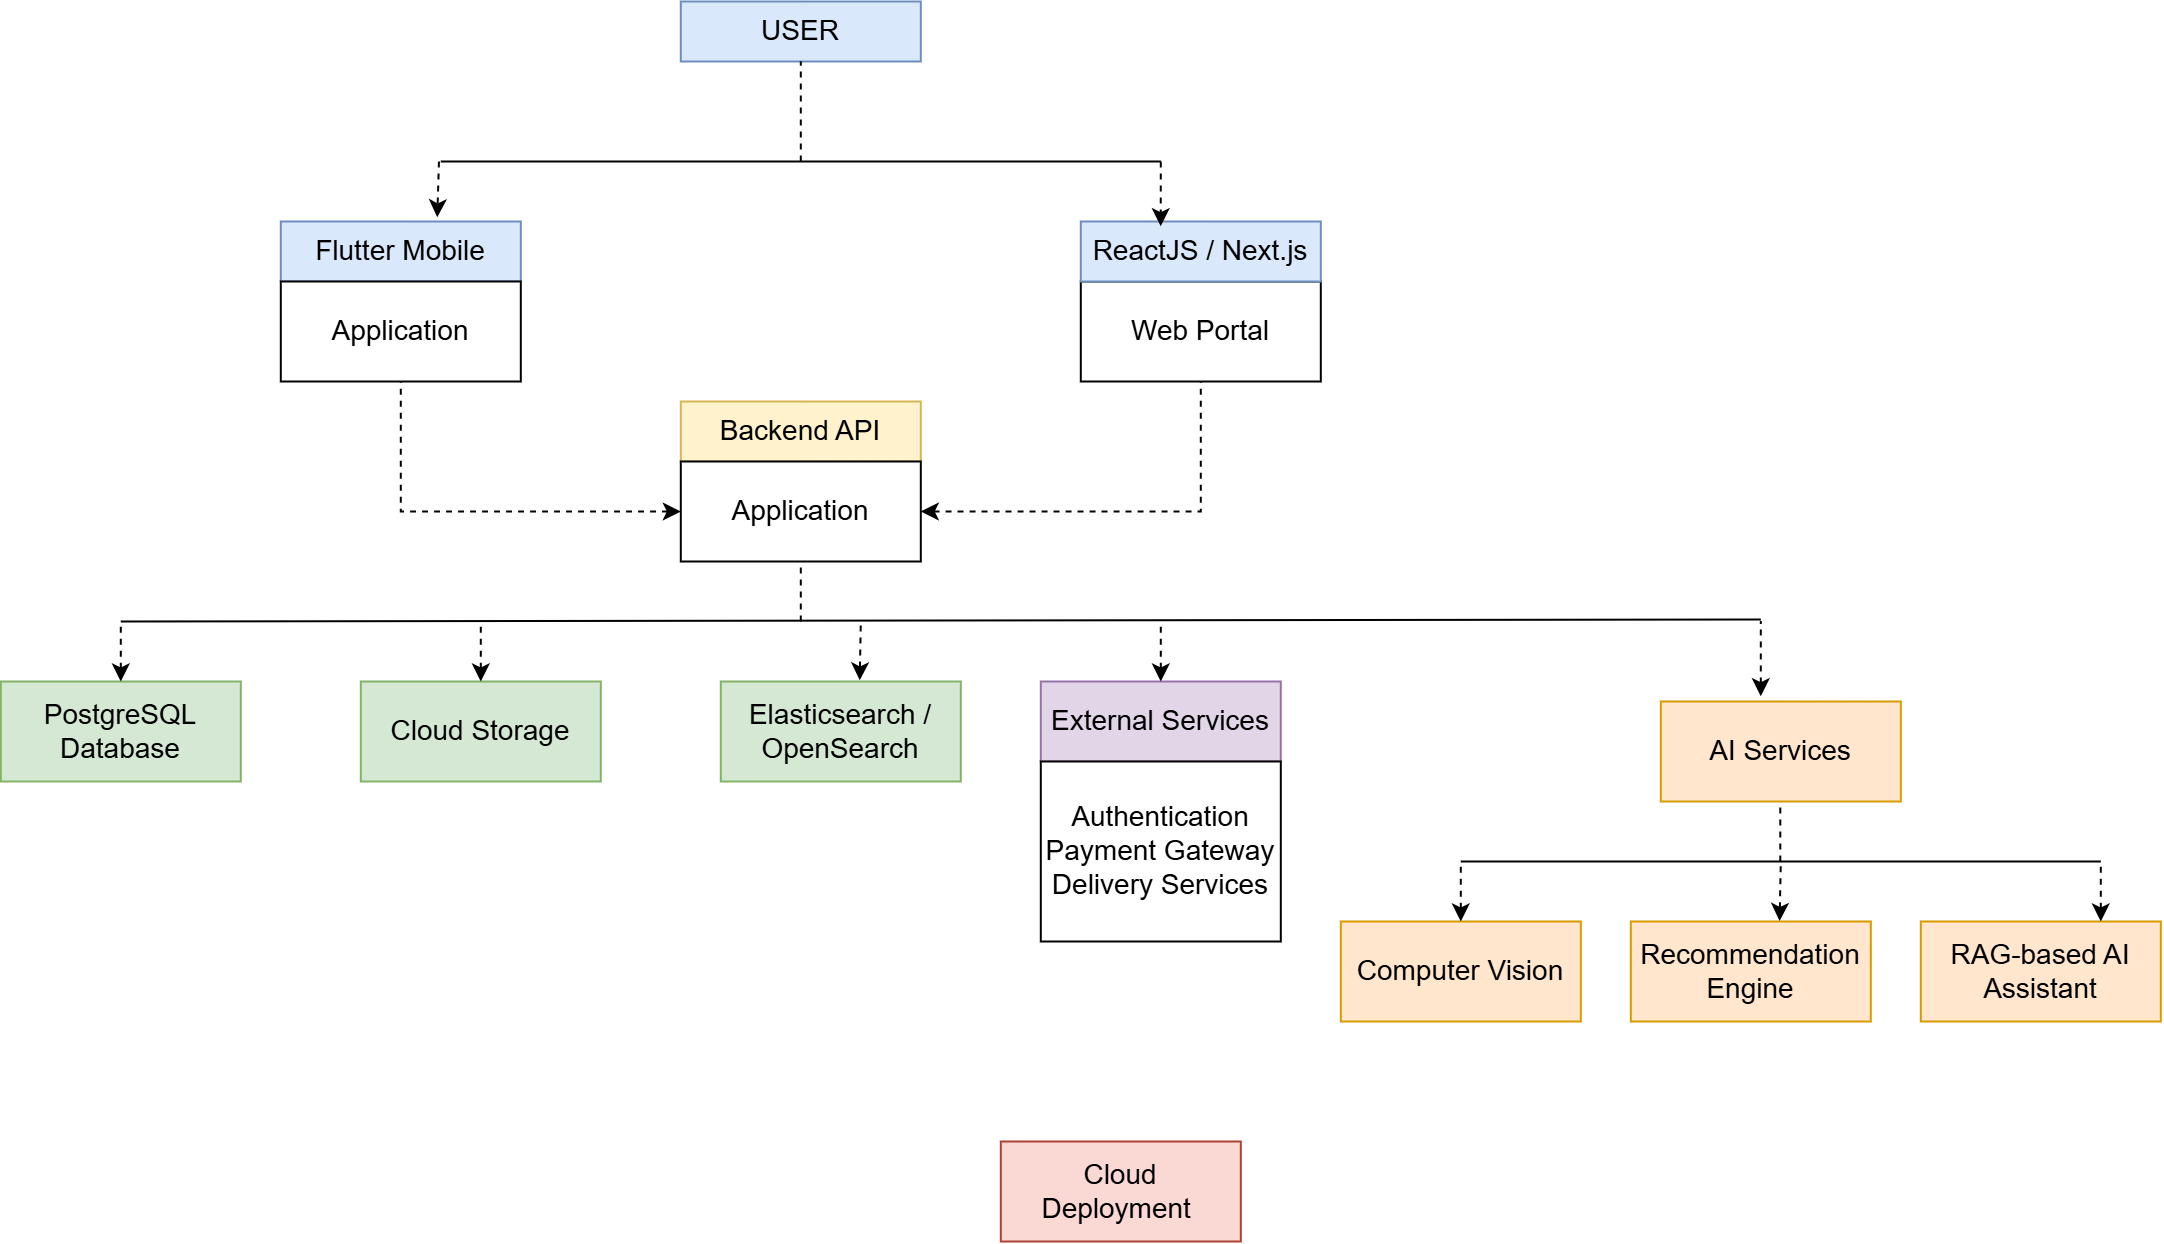
\includegraphics[width=\textwidth,height=0.56\textheight,keepaspectratio]{sections/08-system-architecture.png}
\caption{Proposed system architecture: shared API, data, storage, search, and AI services}
\label{fig:system-architecture}
\end{figure}

\subsection{Component Responsibilities}
\begin{description}[style=nextline]
\item[Client applications] Present discovery, booking, tracking, archive,
marketplace, and administration screens. Validate input for usability and show
loading, empty, and failure states. The API repeats all security-sensitive
validation independently.
\item[Backend API] Authenticate users, enforce role and resource ownership,
validate prices and services, manage the order lifecycle, and record audit
events. PostgreSQL transactions protect related state changes.
\item[PostgreSQL] Store accounts, labs, services, orders, workflow history,
and media metadata. Foreign keys and indexes support consistency and searches.
\item[Object storage] Store original scan files separately from relational
records. Access is private by default; authorized, short-lived links provide
downloads after ownership and order checks.
\item[AI service] Rank labs, retrieve domain knowledge, answer grounded
questions, and analyze scan quality. A backend adapter isolates this service
from public clients and prevents external model keys from reaching browsers.
\item[Search and external adapters] Search indexes, payment providers, and
logistics providers are proposed integration boundaries. They require
independent credentials, failure handling, and contract tests.
\end{description}

\subsection{Core Data Flow and Failure Handling}
A booking request contains selected lab/service identifiers and film details.
The backend validates ownership and availability, derives the charge from the
service catalogue, stores the order, and returns its identifier. Lab staff
advance only allowed status transitions. The status event and current order
state are committed together so a retry cannot silently duplicate a business
event.

For delivery, staff upload a validated file, attach metadata to the correct
order, and publish it after quality checking. The photographer sees only scans
belonging to an authorized order. Failed or incomplete uploads stay unpublished.
Payment and logistics callbacks must be authenticated and idempotent before
they change order state. If the AI service is unavailable, ordinary discovery
and order processing remain usable.

\subsection{Current Repository Boundary}
The diagram is the target design. The current repository implements clients
under \path{apps/}, an Express service under \path{backend/}, and Python AI
modules under \path{ai_service/}. The AI prototype uses local recommendation
data, TF--IDF retrieval, an extractive assistant, and image-quality heuristics.
It does not establish a deployed GPT integration or trained computer-vision
model. The frontend prototypes remain demonstrations until shared backend,
identity, storage, and notification contracts are connected and tested.

%%%%%%%%%%%%%%%%%%%%%%%%%%%%%%%%%%%%%%%%%%%%%%%%%%%%%%%%%%%%
% 3.2.e.10 TECHNOLOGY STACK
% Responsible member: Như Quân
%%%%%%%%%%%%%%%%%%%%%%%%%%%%%%%%%%%%%%%%%%%%%%%%%%%%%%%%%%%%

\section*{3.2.e.10 Technology Stack}
\addcontentsline{toc}{section}{3.2.e.10 Technology Stack}

This section summarizes the proposed technology stack for the
AI-powered Film Photography Platform. The selected technologies
support the development of the mobile application, web portal,
backend services, database, cloud storage, artificial intelligence,
search engine, deployment, and software development workflow.

\begin{table}[htbp]
\centering
\caption{Proposed Technology Stack}
\label{tab:technology-stack}
\begin{tabular}{|p{3.2cm}|p{4.2cm}|p{7.0cm}|}
\hline
\textbf{Category} & \textbf{Technology} & \textbf{Role and Technical Justification} \\
\hline

Mobile Application &
Flutter &
Cross-platform framework for developing the mobile application
for Android and iOS from a shared codebase. It supports the main
photographer and community functions of the platform. \\
\hline

Web Portal &
ReactJS / Next.js &
Used to develop the web portal for Film Lab owners and
administrators. It supports service management, order management,
customer management, reports, and administration functions. \\
\hline

Backend Services &
ASP.NET Core Web API / Node.js (Express) &
Provides business logic, RESTful APIs, authentication,
authorization, database communication, and integration with
external services. \\
\hline

Database &
PostgreSQL &
Relational database for storing structured data such as users,
Film Labs, services, orders, processing status, reviews,
marketplace information, and community data. \\
\hline

Authentication &
JWT / OAuth2 &
Provides secure authentication and authorization. JWT can be used
for authenticated API access, while OAuth2 can support external
authentication and authorization flows. \\
\hline

Cloud Storage &
Azure Blob Storage / Firebase Storage &
Stores digital film scans and other media resources. Cloud storage
supports secure access, backup, recovery, and scalability. \\
\hline

AI Integration &
OpenAI GPT API &
Provides conversational AI capabilities for the AI-powered
Photography Assistant. \\
\hline

AI Framework &
LangChain / Semantic Kernel &
Supports the development and orchestration of AI-powered workflows
and integration with external knowledge and services. \\
\hline

Knowledge Retrieval &
Retrieval-Augmented Generation (RAG) &
Allows the AI Assistant to retrieve relevant photography knowledge
and provide domain-specific responses. \\
\hline

Recommendation &
Recommendation System &
Provides personalized recommendations for Film Labs, services,
film types, and educational resources based on user preferences
and available platform information. \\
\hline

Computer Vision &
Computer Vision Models &
Supports analysis of scanned film images and can be used for
scan-quality evaluation. \\
\hline

Search Engine &
Elasticsearch / OpenSearch &
Provides efficient search for Film Labs, services, marketplace
items, and photography-related knowledge and content. \\
\hline

Cloud Deployment &
Microsoft Azure &
Provides cloud infrastructure for deploying backend services,
storage, databases, and other platform components while supporting
scalability. \\
\hline

CI/CD &
GitHub Actions &
Automates software build, testing, and deployment workflows. \\
\hline

Version Control &
GitHub &
Provides source-code version control, collaboration, change
tracking, and project repository management. \\
\hline

\end{tabular}
\end{table}

\subsection*{Technical Dependencies and Limitations}

The mobile and web applications depend on the Backend API for
business logic and data access. The backend depends on PostgreSQL
for structured data storage and on cloud storage for digital film
scans and other media files.

AI features depend on external AI services and supporting
technologies such as the OpenAI GPT API, LangChain or Semantic
Kernel, RAG, recommendation algorithms, and computer vision
models. Search-related functions depend on Elasticsearch or
OpenSearch.

The final choice between alternative technologies such as
ASP.NET Core Web API and Node.js, ReactJS and Next.js, or
Azure Blob Storage and Firebase Storage should be confirmed
during implementation according to project requirements,
team expertise, integration needs, and deployment constraints.

%%%%%%%%%%%%%%%%%%%%%%%%%%%%%%%%%%%%%%%%%%%%%%%%%%%%%%%%%%%%
% SCRUM-14 DATABASE AND DIGITAL STORAGE ARCHITECTURE
% Responsible member: Nhu Quan
%%%%%%%%%%%%%%%%%%%%%%%%%%%%%%%%%%%%%%%%%%%%%%%%%%%%%%%%%%%%

\subsection{Database and Digital Storage Architecture}

This section defines the proposed database and digital storage architecture
for the AI-powered Film Photography Platform.

\subsubsection{Database Architecture}

PostgreSQL is proposed as the primary relational database for storing
structured system data. The database stores information related to users,
films, Film Labs, services, orders, reviews, community activities, and
film scan metadata.

The Backend API acts as the main access layer between the mobile/web
applications and PostgreSQL. Client applications send API requests to the
Backend API, which handles business logic, authentication, authorization,
and database access.

The main data entities include:

\begin{itemize}
    \item User
    \item Film
    \item Film Lab
    \item Service
    \item Order
    \item Review
    \item Community
    \item Film Scan Metadata
\end{itemize}

\subsubsection{Digital Storage Architecture}

Digital film scans are separated from structured relational data.
PostgreSQL stores scan metadata such as file name, file type, file size,
file path, and related information, while the actual film scan files are
stored in cloud storage.

The proposed architecture uses the Backend API as the access layer for
uploading and retrieving film scans. This approach separates structured
data management from large media file storage and supports scalability
and secure file access.

\subsubsection{Data Access and Security}

The Backend API controls access to both PostgreSQL and cloud storage.
Authentication and authorization mechanisms are applied before users can
access protected data or digital film scans.

This architecture provides centralized data access, supports backup and
recovery, and allows the storage system to scale as the number of users
and film scans increases.

\begin{figure}[htbp]
    \centering
    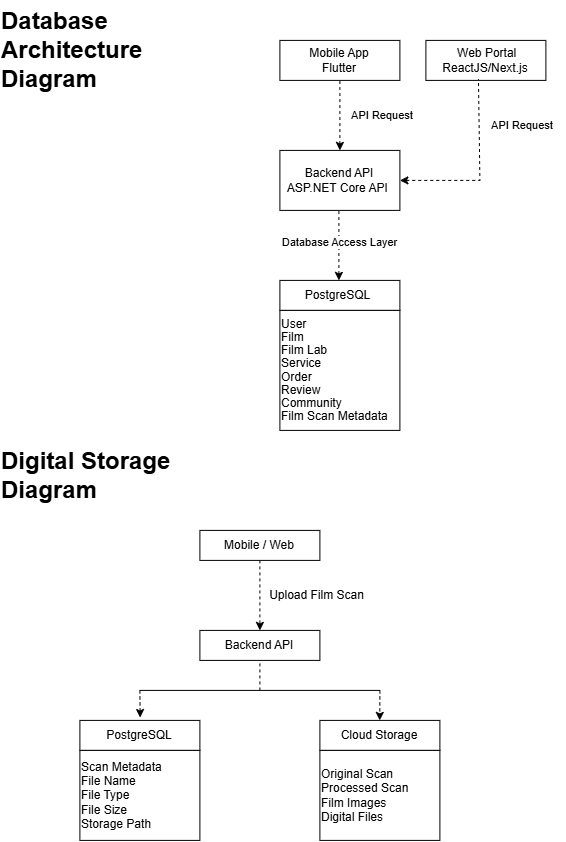
\includegraphics[width=0.85\textwidth]{sections/14-database-storage-architecture.png}
    \caption{Database and Digital Storage Architecture}
    \label{fig:database-storage-architecture}
\end{figure}

\clearpage
\section{Implemented Data Model and API Contracts}
The earlier database/storage diagram describes the target platform. This
section documents the smaller executable baseline in \path{backend/schema.sql}
and \path{backend/server.js}. It prevents planned entities from being mistaken
for tables already available in the submission.

\subsection{Current Entity Relationships}
\begin{figure}[htbp]\centering
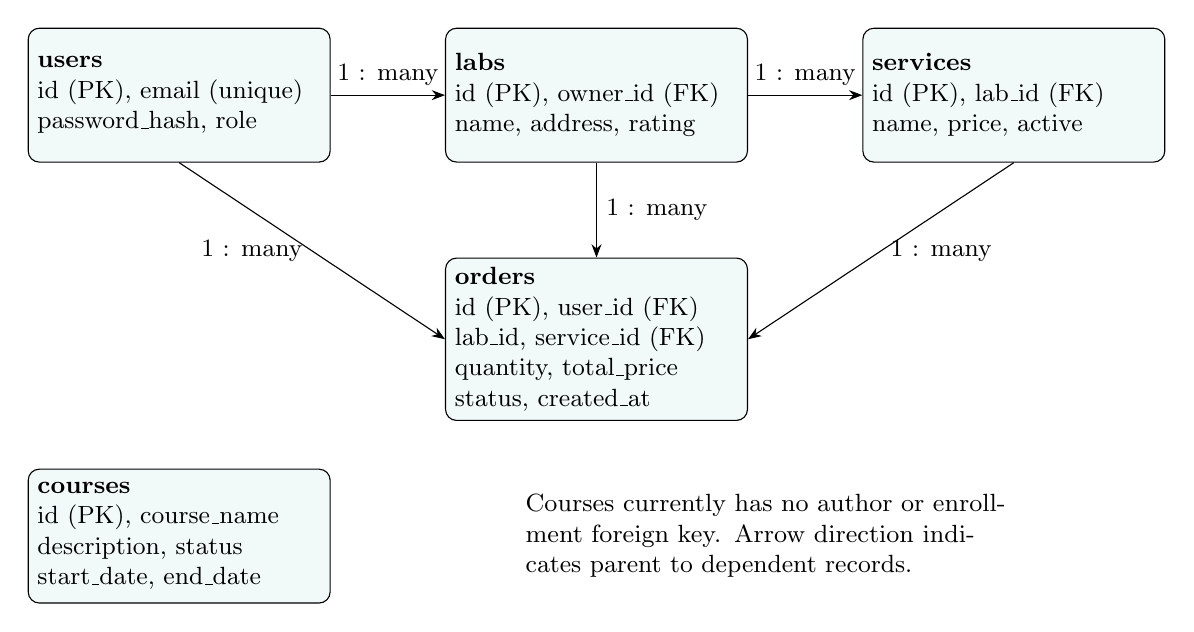
\begin{tikzpicture}[x=1cm,y=1cm,font=\small,
 entity/.style={draw,rounded corners,fill=teal!5,text width=3.6cm,align=left,minimum height=17mm},>=Stealth]
\node[entity] (users) at (0,0) {\textbf{users}\\id (PK), email (unique)\\password\_hash, role};
\node[entity] (labs) at (5.3,0) {\textbf{labs}\\id (PK), owner\_id (FK)\\name, address, rating};
\node[entity] (services) at (10.6,0) {\textbf{services}\\id (PK), lab\_id (FK)\\name, price, active};
\node[entity] (orders) at (5.3,-3.1) {\textbf{orders}\\id (PK), user\_id (FK)\\lab\_id, service\_id (FK)\\quantity, total\_price\\status, created\_at};
\node[entity] (courses) at (0,-5.6) {\textbf{courses}\\id (PK), course\_name\\description, status\\start\_date, end\_date};
\draw[->] (users)--node[above]{1 : many}(labs);
\draw[->] (labs)--node[above]{1 : many}(services);
\draw[->] (users.south)--node[left]{1 : many}(orders.west);
\draw[->] (labs.south)--node[right]{1 : many}(orders.north);
\draw[->] (services.south)--node[right]{1 : many}(orders.east);
\node[align=left,text width=6.2cm] at (7.5,-5.6) {Courses currently has no author or enrollment foreign key. Arrow direction indicates parent to dependent records.};
\end{tikzpicture}
\caption{ERD derived from the current five-table bootstrap schema}
\end{figure}

\subsection{Constraints and Data Dictionary}
\begin{longtable}{p{0.20\textwidth}p{0.70\textwidth}}
\toprule\textbf{Entity / field} & \textbf{Meaning and implemented constraint}\\\midrule\endhead
users & Unique, non-null email; non-null password hash. Roles: photographer, lab\_owner, expert, moderator, admin. Employee/delivery identities are not yet implemented.\\
labs & owner\_id references users; name/address required; rating is between 0 and 5 and starts at 0. API role validation controls creation, while SQL only checks the owner exists.\\
services & Belongs to a lab; positive integer-valued NUMERIC price; active flag controls availability for order creation. Price is interpreted as VND by the current application.\\
orders & User, lab and service references required; quantity 1--100; positive total; timestamp defaults to database time. API verifies service/lab association. Separate foreign keys alone do not enforce that association for arbitrary SQL writes.\\
order status & Database text defaults to pending; no SQL transition constraint. The browser demo has its own six-state enum; it is not synchronized with this field.\\
courses & Status limited to draft, published or cancelled; end date cannot precede start date. No participant or capacity table exists yet.\\
Indexes & orders(user\_id) supports ownership filtering; services(lab\_id) supports service lookup. These are definitions, not benchmark evidence.\\
\bottomrule
\end{longtable}
The bootstrap is for a new local database. Existing team databases require
reviewed migrations and backup. Scan, payment, pickup, moderation, event
registration and server audit tables remain additions to the target design.

\subsection{Current HTTP Contract}
Development base URL: \url{http://127.0.0.1:3000}. Protected calls use
\texttt{Authorization: Bearer <token>}. Login returns a one-hour HS256 token;
both signing and verification read the same secret of at least 32 characters.
\begin{longtable}{p{0.28\textwidth}p{0.29\textwidth}p{0.32\textwidth}}
\toprule\textbf{Endpoint} & \textbf{Access / input} & \textbf{Successful response}\\\midrule\endhead
POST /auth/login & email, password; public & 200: message, token, user(id,email,role).\\
GET /labs; /courses & Any valid user token & 200: database row array. Course listing currently includes all statuses; publication filtering is future work.\\
GET /orders & Any valid token & 200: own orders; admin can list all. This is not a lab-staff assignment query.\\
POST /labs & lab\_owner/admin; name, address, optional description & 200: created row, owner from token and rating 0.\\
POST /courses & expert/admin; course\_name, description, status, start\_date, end\_date & 200: created course row.\\
POST /orders & photographer/admin; integer lab\_id, service\_id, quantity & 200: created pending order; total from active service price times quantity.\\
GET /users; /users/full & admin & 200: id, email, role only; /users/full limits results to five.\\
GET /tables; /schema/:table & admin & 200: table or column metadata; intended for development inspection.\\
\bottomrule
\end{longtable}
Malformed JSON or invalid fields return 400; invalid/missing credentials return
401; an authenticated but disallowed role returns 403. Database failures return
a generic 500 message. Existing creation routes return 200, not 201; documentation
records the actual implementation rather than assuming a different contract.

\textbf{Order example (illustrative, requires seeded IDs):}
\begin{verbatim}
POST /orders
Authorization: Bearer <token>
Content-Type: application/json

{"lab_id": 1, "service_id": 2, "quantity": 3}
\end{verbatim}
If the selected service costs 120,000 VND, the persisted total is 360,000 VND.
The example is arithmetic and a contract illustration, not a captured live
database response. No endpoint accepts the browser's local storage snapshot as
trusted authorization or order data.

\subsection{Integration Decisions and Remaining Contracts}
\begin{description}[style=nextline]
\item[Current stack] React/TypeScript/Vite, Flutter sources, Express/PostgreSQL
and a separate Python AI service are present. Next.js, ASP.NET Core, OAuth2,
hosted GPT and managed search listed earlier are candidate technologies, not
additional installed implementations.
\item[Private scan design] Target storage keeps file bytes separate from SQL
metadata. An authorized API should issue short-lived access, verify upload
completion and publish metadata transactionally. The current demo stores only
file name, size and type; it does not implement this storage protocol.
\item[Status integration] Agree a shared order enum, allowed transition table,
resource ownership checks and concurrency/version behavior before connecting
the frontend. Preserve physical processing detail in history even if the UI
groups stages into simpler labels.
\item[Transaction boundaries] Reservation, pickup, payment and notification need
idempotency and failure recovery contracts. A browser success message is not
evidence of a committed external transaction.
\end{description}

\clearpage
% ============================================================
% MOBILE AND WEB DESIGN
% Responsible member: Nguyen Dao Quoc Khanh
% ============================================================

\section{Mobile and Web Design}

This section presents the proposed user interfaces for the Photographer Mobile
Application, Film Lab Web Portal, Administration Web Portal, Marketplace, and
Digital Film Archive. Flutter is proposed for the mobile application, while
ReactJS or Next.js is proposed for the web portals.

\subsection{UI/UX Guidelines}

The interfaces follow these common guidelines:

\begin{itemize}
    \item The mobile application uses simple bottom navigation for Home,
    Orders, Archive, Marketplace, and Profile.
    \item The Film Lab and Administration portals use a consistent sidebar,
    page header, searchable tables, filters, and pagination.
    \item Each screen has one clear primary action, such as booking a service,
    updating an order status, or uploading scan files.
    \item Order states use both color and text labels. Important examples are
    Pending, Processing, Scanning, Ready for Delivery, and Completed.
    \item Forms show visible labels and short validation messages without
    removing valid information entered by the user.
    \item Loading, empty, success, confirmation, and error states are provided
    for important actions.
    \item Destructive actions and actions that affect another user require a
    confirmation step.
    \item Mobile and web layouts remain readable on their supported screen
    sizes and provide keyboard focus for web controls.
\end{itemize}

\subsection{Photographer Mobile Application}

The Photographer Application is developed with Flutter for Android and iOS.
It allows photographers to find a Film Lab, create processing orders, track
their film, receive scan files, use the Marketplace, and manage a personal
Digital Film Archive.

\begin{table}[htbp]
\centering
\small
\renewcommand{\arraystretch}{1.1}
\caption{Main Photographer Mobile Application Screens}
\label{tab:photographer-mobile-screens}
\begin{tabular}{|p{3.4cm}|p{9.2cm}|}
\hline
\textbf{Screen Group} & \textbf{Main Functions} \\
\hline
Authentication & Register, log in, reset password, and verify an account. \\
\hline
Home & Show current orders, nearby Film Labs, recommendations, and
notifications. \\
\hline
Film Lab Discovery & Search and filter by location, film format, service,
price, rating, and processing time. \\
\hline
Booking & Select a service, enter film information, choose pickup or drop-off,
review the cost, and confirm the order. \\
\hline
Orders & Display order history and the processing status timeline. \\
\hline
Scan Delivery & Preview thumbnails, download scan files, and save photographs
to the archive. \\
\hline
Marketplace and Community & View listings and community content, contact
sellers, and report inappropriate content. \\
\hline
AI Assistant & Ask questions about film stocks, exposure, camera settings,
Film Labs, and processing services. \\
\hline
Profile & Update personal details, saved addresses, notifications, and account
settings. \\
\hline
\end{tabular}
\end{table}

The main booking flow is:

\begin{center}
\texttt{Login $\rightarrow$ Search Film Lab $\rightarrow$ Compare Services
$\rightarrow$ Enter Film Details $\rightarrow$ Choose Pickup
$\rightarrow$ Confirm Order $\rightarrow$ Track Status}
\end{center}

Before confirmation, the application displays the service price, pickup fee,
estimated completion time, and total amount. If location permission is not
available, the photographer can manually enter a district or city.

\subsection{Film Lab Web Portal}

The Film Lab Web Portal gives owners and employees a larger workspace for
handling orders and scan files. A Lab owner can manage the Film Lab profile,
services, prices, employees, and reports. A Lab employee can process assigned
orders and upload scan files.

The main pages are Dashboard, Orders, Order Details, Processing Board,
Schedule, Scan Delivery, Services and Pricing, Customers, Reports, and Lab
Settings. The processing workflow is:

\begin{center}
\texttt{New Order $\rightarrow$ Accepted $\rightarrow$ Film Received
$\rightarrow$ Developing $\rightarrow$ Scanning $\rightarrow$
Quality Checking $\rightarrow$ Scans Published $\rightarrow$ Completed}
\end{center}

Every status update records the employee, update time, and an optional note.
Invalid status jumps are disabled. During scan delivery, the portal validates
file type and size, displays upload progress, supports retry, and requires a
final confirmation before publishing files to the photographer.

\subsection{Administration Web Portal}

The Administration Portal supports system administrators, moderators, finance
staff, and support staff. Role-based permissions limit each user to the data
and actions required for their work.

The portal provides the following main functions:

\begin{itemize}
    \item manage users, roles, account status, and Film Lab applications;
    \item manage service categories, platform fees, and public settings;
    \item monitor payments, failed transactions, refunds, and activity;
    \item review community content, marketplace listings, complaints, and
    disputes;
    \item view reports and search the administrative audit log.
\end{itemize}

For Film Lab approval, an administrator checks the submitted business and
service information, requests missing information when necessary, and records
an approval or rejection reason. Important access, moderation, payment, and
configuration actions are written to the audit log.

\subsection{Marketplace Interface}

The Marketplace supports cameras, lenses, film rolls, accessories, and other
film photography equipment. Users can search by keyword and filter by category,
brand, condition, location, price, and listing date.

The main screens are Marketplace Home, Search Results, Listing Details, Create
Listing, Seller Profile, Messages, Saved Items, My Listings, and Transactions.
A seller creates a listing using the following flow:

\begin{center}
\texttt{Select Category $\rightarrow$ Upload Photos $\rightarrow$
Enter Item Details $\rightarrow$ Set Price and Delivery
$\rightarrow$ Preview $\rightarrow$ Submit}
\end{center}

The interface clearly marks Draft, Active, Reserved, Sold, Hidden, Rejected,
and Expired listings. Users can report suspicious listings, messages, or
accounts, and the report is sent to the Administration Portal.

\subsection{Digital Film Archive Interface}

The Digital Film Archive stores scan files published by Film Labs and helps the
photographer organize them by order, album, film stock, shooting date, tags,
and favorite status.

The archive includes a library, order scan view, photo viewer, album manager,
search and filters, metadata editor, downloads, and storage and privacy
settings. Film Lab metadata, such as order code, scanner, resolution, and
delivery date, is separated from personal metadata entered by the photographer.
Changing an album, tag, or note does not overwrite the original delivered file.

New scan deliveries are private by default. Sharing requires a separate user
action. Large downloads show progress and can be retried if the network is
interrupted.

\subsection{Frontend Component Architecture}

The Flutter application and ReactJS or Next.js portals use the same separation
of responsibilities.

\begin{table}[htbp]
\centering
\small
\renewcommand{\arraystretch}{1.1}
\caption{Frontend Architecture Layers}
\label{tab:frontend-architecture-layers}
\begin{tabular}{|p{3.2cm}|p{9.4cm}|}
\hline
\textbf{Layer} & \textbf{Responsibility} \\
\hline
Presentation & Screens, pages, layouts, forms, tables, dialogs, and reusable
interface components. \\
\hline
State and Feature & Authentication, order, marketplace, archive, profile, and
notification state. \\
\hline
Domain & Shared models and application rules for users, Film Labs, services,
orders, scans, and listings. \\
\hline
API and Service & REST API communication, file upload and download, and
real-time updates. \\
\hline
Shared & Theme, routing, form validation, error mapping, localization, and
common utilities. \\
\hline
\end{tabular}
\end{table}

A user action starts in the presentation layer. The feature state validates the
input and calls the relevant service. The service communicates with the backend
or file storage and returns a shared model. Finally, the state is updated and
the interface shows the result. Screens do not store secrets or call backend
endpoints directly.

\subsection{Main Cross-Platform UI Flow}

The main interaction between the mobile and web interfaces is summarized as
follows:

\begin{enumerate}
    \item The photographer searches for a Film Lab and creates an order in the
    mobile application.
    \item Film Lab staff review the order and update its processing stages in
    the web portal.
    \item Status notifications are displayed in the Photographer Application.
    \item The Film Lab uploads and publishes scan files after quality checking.
    \item The photographer previews, downloads, and organizes the scans in the
    Digital Film Archive.
    \item Reports or disputes are transferred to the Administration Portal for
    review.
\end{enumerate}

\subsection{Frontend Sequence Summaries}

Four frontend sequence diagrams are planned for implementation and
presentation:

\begin{enumerate}
    \item \textbf{Create service order:} the Photographer App validates the
    booking, sends it to the Platform API, and displays the returned order code.
    \item \textbf{Update processing status:} the Film Lab Portal sends the next
    status to the API, which records the history and notifies the photographer.
    \item \textbf{Publish scans:} the Film Lab Portal uploads files to storage,
    saves metadata through the API, and makes the files available in the mobile
    application.
    \item \textbf{Moderate a listing:} the Administration Portal retrieves the
    report and evidence, records the decision, updates the Marketplace, and
    writes an audit event.
\end{enumerate}

\subsection{Initial Wireframes and Presentation Plan}

The first wireframes should show Photographer Home, Film Lab Search, Film Lab
Details, Booking, Order Tracking, Scan Delivery, Film Lab Dashboard, Processing
Board, Scan Upload, Admin Moderation, Marketplace Search, Listing Details,
Archive Library, and Photo Viewer.

During the presentation, the UI flow should be introduced first, followed by
one mobile example, one web portal example, the component architecture, and the
scan delivery sequence. The recommended speaking time for this section is four
to five minutes.

\clearpage
\chapter{Prototype Handover and Verification}
\section{Repository Deliverables}
\begin{longtable}{p{0.22\textwidth}p{0.34\textwidth}p{0.35\textwidth}}
\caption{Evidence and implementation boundaries}\label{tab:submission-evidence}\\
\toprule
\textbf{Deliverable} & \textbf{Repository evidence} & \textbf{Boundary}\\
\midrule\endfirsthead
\toprule\textbf{Deliverable} & \textbf{Repository evidence} & \textbf{Boundary}\\\midrule\endhead
Mobile app & \path{apps/mobile/lib/}, \path{apps/mobile/test/} & Flutter source and demonstration data; device build and shared API integration require separate evidence.\\
Web portals & \path{apps/web/src/}, \path{apps/web/package.json} & React/TypeScript interface for lab and admin workflows; local demonstration state.\\
Business API & \path{backend/server.js}, \path{backend/authMiddleware.js} & Express endpoints with PostgreSQL dependency; configured database and integration tests are required.\\
AI prototype & \path{ai_service/}, \path{ai_service/openapi.json} & Local recommendation, retrieval, grounded extraction, and scan-quality heuristics.\\
AI validation & \path{tests/}, \path{scripts/evaluate_ai.py}, \path{scripts/smoke_test.py} & Automated tests and reproducible evaluation scripts; synthetic/local results do not demonstrate production quality.\\
Deployment design & \path{Dockerfile}, \path{infra/azure/}, \path{.github/workflows/} & Container, infrastructure, and workflow definitions; presence of files is not proof of a live deployment.\\
Design report & \path{CNPM_Report.tex}, \path{sections/}, \path{docs/} & Consolidated requirements, responsibilities, architecture, interface flows, and submission evidence.\\
\bottomrule
\end{longtable}

\section{Demonstration Procedure}
\begin{enumerate}
\item Install the web dependencies in \path{apps/web/} with
\texttt{npm ci}; run \texttt{npm run build} and \texttt{npm run dev}.
Open the local address printed by Vite.
\item Demonstrate Film Lab and Admin portal navigation, order search/filtering,
processing stages, marketplace/archive views, and available form validation.
Describe each operation as a local prototype action unless a verified API
response and persistent database result are shown.
\item For mobile, install a compatible Flutter SDK, run
\texttt{flutter pub get}, \texttt{flutter analyze}, and \texttt{flutter test}
inside \path{apps/mobile/}. Launch a supported device target with
\texttt{flutter run}. Source inspection alone is not a device test.
\item From the repository root, install Python project dependencies and run
\texttt{python -m unittest discover -s tests -v}. Start the AI adapter with
\texttt{python -m ai\_service.api}; use \path{/health}, \path{/ready}, and
\path{/openapi.json} to inspect its contract.
\item Present one supported photography question, one unsupported question,
and one recommendation request. Explain the local knowledge/data boundary and
show how insufficient evidence is reported.
\item Open this report and the acceptance/submission documents in \path{docs/}.
Relate each demonstrated feature to the relevant requirement and work item.
\end{enumerate}

\section{Acceptance and Remaining Integration Work}
For each requirement, record its identifier, owner, code or document path,
test procedure, observed result, and unresolved dependency. A feature is
complete only when its agreed acceptance criteria have supporting evidence.
Interface mockups, implemented local interactions, automated unit tests, and
verified end-to-end operations are distinct evidence levels.

Before claiming the complete platform is operational, the team must verify:
\begin{itemize}
\item database schema and repeatable migrations, seeded non-sensitive test
data, configured secrets, and authorization for each protected resource;
\item mobile/web authentication and shared API integration, including
cross-user isolation, failure states, and persistence after reload;
\item private cloud uploads, ownership checks, scan publication and downloads;
\item real payment, logistics, and notification adapters, or an explicitly
documented decision to exclude them from the assessed prototype;
\item supported-device mobile builds, end-to-end tests, accessibility checks,
and performance/recovery measurements against the proposed targets;
\item deployment health, backup and restore verification, and reproducible
release configuration before calling the system production ready.
\end{itemize}

\section{Contribution and Submission Evidence}
The source repository is the primary record of implemented changes. Each
meaningful commit should describe a coherent change and, where available,
reference its Jira issue. Jira items should link to the resulting code,
document, test evidence, or demonstration and describe unresolved dependencies.
Only move an item to Done when its actual acceptance criteria are satisfied.

Contributor graph height is a count-based view of eligible commits in its
selected period. It does not measure feature completeness or the quality of a
member's work. The submission should explain ownership with requirements,
implemented artifacts, tests, and review evidence, without representing planned
work as completed work.

\clearpage
\section{Verification Snapshot}
The submission snapshot was checked on Windows using Node.js 24.19 and the
bundled Python environment on 17 September 2026. The web production build and
TypeScript compilation succeeded. The automated suites passed 41 AI tests,
9 web-domain tests, and 11 backend authorization/validation tests. Backend tests
use an isolated database stub; no live PostgreSQL or cloud deployment is claimed.

\begin{longtable}{p{0.20\textwidth}p{0.43\textwidth}p{0.27\textwidth}}
\toprule\textbf{Area} & \textbf{Verification evidence} & \textbf{Result / limitation}\\\midrule\endhead
AI & Recommendation constraints, retrieval, refusal on insufficient evidence, scan quality and HTTP contracts & 41 tests passed; local and synthetic datasets.\\
Web domain & Order transitions, service validation, scan boundaries, publication, approval/moderation, CSV safety and saved-state round trip & 9 tests passed.\\
Business API & Shared JWT key, malformed/expired/forged tokens, role checks, private order listing, safe login and server-derived order prices & 11 tests passed; database stub.\\
React build & TypeScript and Vite production output & Passed.\\
Mobile & Source and navigation/widget test inspected; booking estimate and demo wording corrected & Flutter SDK unavailable locally; device build not verified.\\
Report & LaTeX sources consolidated and compiled using Tectonic & PDF generated; visual review required for release.\\
\bottomrule
\end{longtable}

\section{Requirement-to-Code Examples}
\begin{description}[style=nextline]
\item[US-03 / SCRUM-29: inspect an order] A lab operator can search by order,
customer or service and filter by status. \path{apps/web/src/App.tsx} contains
the order table, selection and detail view. Keyboard Enter selects a row.
\item[US-04: advance a workflow] \path{apps/web/src/domain.ts} permits only
the next stage. Completed orders cannot advance, and scan orders at quality
check require reviewed publication before completion.
\item[US-05: deliver scans] JPEG/TIFF extension and MIME checks, positive size,
50 MB per-file limit, duplicate filenames and a 100-file limit are enforced.
The demo saves private metadata after quality and release confirmation;
actual file bytes remain on the device.
\item[US-08 and US-09 / SCRUM-30: administration] Incomplete lab applications
cannot be approved. Rejections and moderation decisions require reasons.
Repeated final decisions are rejected and local audit entries record changes.
Browser audit data is not tamper-proof server evidence.
\item[Security boundary] The Express API shares one configured signing and
verification secret, restricts user/schema inspection to administrators, and
filters non-admin orders by owner. Order totals come from the service catalogue.
\end{description}

\section{Workflow and Sequence Diagrams}
The diagrams below distinguish implemented local interactions from the target
integration design. The complete story/rule matrix and manual checklist are in
\path{docs/AcceptanceTraceability.md} and \path{docs/SubmissionChecklist.md}.

\begin{figure}[htbp]\centering
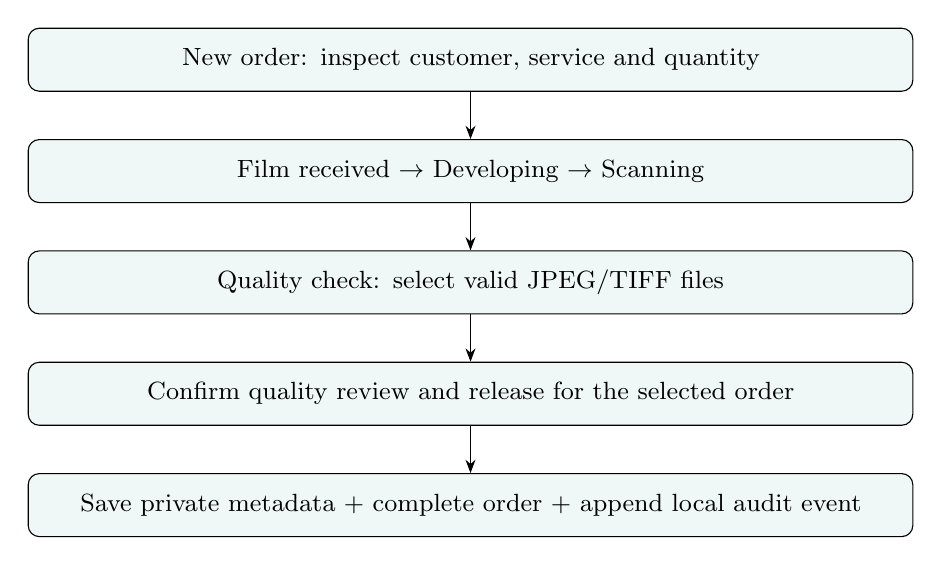
\begin{tikzpicture}[node distance=6mm, box/.style={draw,rounded corners,fill=teal!6,text width=11cm,align=center,minimum height=8mm,font=\small}, >=Stealth]
\node[box] (a) {New order: inspect customer, service and quantity};
\node[box,below=of a] (b) {Film received $\rightarrow$ Developing $\rightarrow$ Scanning};
\node[box,below=of b] (c) {Quality check: select valid JPEG/TIFF files};
\node[box,below=of c] (d) {Confirm quality review and release for the selected order};
\node[box,below=of d] (e) {Save private metadata + complete order + append local audit event};
\draw[->] (a)--(b);\draw[->] (b)--(c);\draw[->] (c)--(d);\draw[->] (d)--(e);
\end{tikzpicture}
\caption{Implemented local web workflow; no cloud upload or customer message is sent}
\end{figure}

\begin{figure}[htbp]\centering
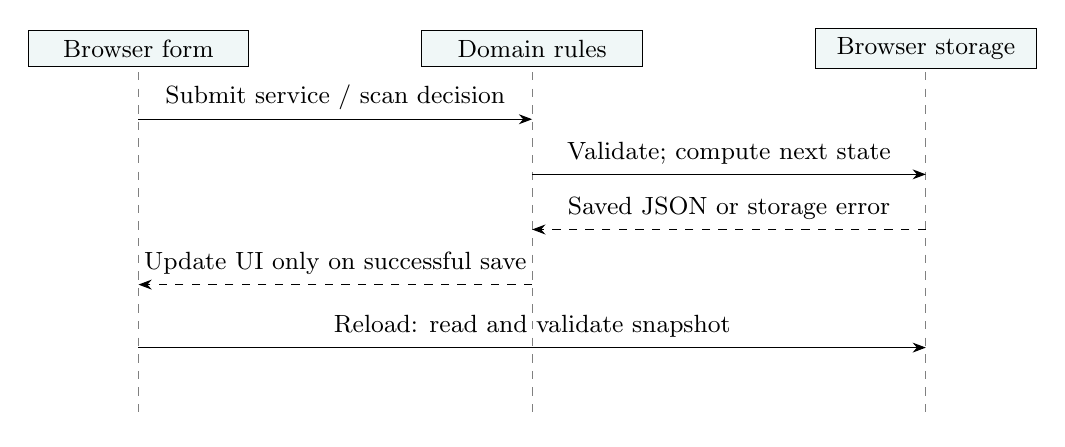
\begin{tikzpicture}[x=1cm,y=1cm,>=Stealth,font=\small]
\node[draw,fill=teal!6,minimum width=2.8cm] at (0,0) {Browser form};
\node[draw,fill=teal!6,minimum width=2.8cm] at (5,0) {Domain rules};
\node[draw,fill=teal!6,minimum width=2.8cm] at (10,0) {Browser storage};
\foreach \x in {0,5,10}{\draw[dashed,gray] (\x,-0.3)--(\x,-4.7);}
\draw[->] (0,-0.9)--node[above]{Submit service / scan decision}(5,-0.9);
\draw[->] (5,-1.6)--node[above]{Validate; compute next state}(10,-1.6);
\draw[->,dashed] (10,-2.3)--node[above]{Saved JSON or storage error}(5,-2.3);
\draw[->,dashed] (5,-3.0)--node[above]{Update UI only on successful save}(0,-3.0);
\draw[->] (0,-3.8)--node[above]{Reload: read and validate snapshot}(10,-3.8);
\end{tikzpicture}
\caption{Implemented state persistence, validation and error handling in the web demo}
\end{figure}

\clearpage
\section{Known Limits and Demonstration Talking Points}
The assessed implementation is a documented prototype with executable local
interactions and testable backend/AI modules. It is not a completed production
marketplace. Shared frontend authentication, live database migration verification,
cross-device synchronization, cloud scan storage, payment/logistics adapters,
mobile device testing and deployment remain explicit integration tasks.

For a five-minute demonstration: introduce the problem and actors; show order
search and a valid status transition; demonstrate a service edit that survives
reload; show scan validation and private publication metadata; demonstrate an
admin decision and its audit event; finish with the test summary and the
requirement-to-code matrix. Explain that local role switching is a demonstration
control and that backend authorization must independently enforce permissions.

\clearpage
\section{Measurable Quality Acceptance Plan}
The following thresholds are proposed engineering targets for team review,
not an official lecturer rubric, measured service levels or completed tests.
They make the broad non-functional requirements assessable in a later
integration milestone.
\begin{longtable}{p{0.14\textwidth}p{0.43\textwidth}p{0.33\textwidth}}
\toprule\textbf{ID / area} & \textbf{Proposed acceptance criterion} & \textbf{Method / current evidence}\\\midrule\endhead
NFR-01 Security & All protected endpoints reject absent/invalid tokens; forbidden role/resource access cannot read or mutate data. & Negative HTTP cases and cross-user tests. Eleven backend tests provide partial evidence, with a DB stub.\\
NFR-02 Performance & With 10,000 seeded labs and 50 concurrent clients, discovery API p95 below 2 s and error rate below 1\% during a 10-minute run. & Record hardware, dataset, warm-up, latency distribution and errors. Not run.\\
NFR-03 Reliability & Restart after an acknowledged order write preserves that order; retrying the same booking key produces one order. & Kill/restart plus duplicate-request integration test. Persistence/idempotency not verified.\\
NFR-04 Recovery & Proposed development recovery objective: at most 24 h data loss and restoration within 4 h. & Restore a backup into an isolated DB and verify row/file ownership counts. Not run.\\
NFR-05 Privacy & Customer A cannot obtain customer B's scan metadata or file bytes; new deliveries default private. & API and storage authorization tests, including expired links. Only local metadata privacy is tested.\\
NFR-06 Usability & Core forms usable by keyboard; required actions reachable at 360 px and 1280 px widths without clipped controls. & Manual focus, labels, validation, narrow-screen review. No complete accessibility audit claimed.\\
NFR-07 Integrity & Concurrent reservations cannot oversell; invalid quantity, lab/service mismatch and dates are rejected. & API unit tests cover part of validation; concurrent DB transactions remain untested.\\
NFR-08 Maintainability & A fresh checkout installs from lockfiles and passes TypeScript build and deterministic unit suites. & npm ci and web build passed; 61 automated tests passed. Flutter execution is pending.\\
NFR-09 AI behavior & Unsupported questions disclose insufficient evidence; recommendations respect explicit hard constraints. & Existing local AI tests cover constrained behavior; results are not a general model-accuracy benchmark.\\
\bottomrule
\end{longtable}

\section{Acceptance Traceability}
Detailed stories and manual TC identifiers are maintained in
\path{docs/AcceptanceTraceability.md} and \path{docs/SubmissionChecklist.md}.
The matrix below is a compact assessment guide; ``local'' always means one
browser using demonstration data.
\begin{longtable}{p{0.19\textwidth}p{0.31\textwidth}p{0.40\textwidth}}
\toprule\textbf{Requirement} & \textbf{Artifact / Jira} & \textbf{Evidence and status}\\\midrule\endhead
UC-01 / US-01 & Mobile Home; SCRUM-5/28 & Search/filter source exists. Flutter runtime unverified; AI tests are independent of mobile.\\
UC-02 / US-02 & Mobile preview, POST /orders; SCRUM-6/28 & Preview pricing corrected; API quantity/price tested with stub. Full booking flow not integrated.\\
UC-03 / US-03/04 & Web Orders and domain; SCRUM-8/29 & Search/details and permitted local transitions; domain tests pass. No mobile synchronization.\\
UC-04 / US-05/06 & ScanDelivery, Archive; SCRUM-9/29/31 & Validation/publication logic tested; picker automation blocked. No cloud delivery/download proof.\\
UC-05 / US-07/08 & Marketplace, Moderation; SCRUM-10/30/31 & Local listing decisions and audit rules tested. No completed purchase/payment.\\
UC-06 / BR-08 & FunctionalRequirements; course API & Six-flow specification exists. Registration, capacity and article discussion remain planned.\\
US-09 / BR-07 & ApprovalsPage; SCRUM-30 & Incomplete applications blocked; reason requirements tested. No server approval workflow.\\
US-10 & Theme/styles and form components; SCRUM-27 & Explicit empty/error/focus states; complete usability assessment pending.\\
US-11 / BR-09 & Mobile assistant and Python AI; SCRUM-28 & Mobile responses are samples. Python tests cover independent retrieval/recommendation behavior.\\
US-12 & Report, diagrams, matrix; SCRUM-4/26/32 & Source paths, use cases, schema and verification connected in the document package.\\
\bottomrule
\end{longtable}

\section{Release Checklist and Risks}
\begin{enumerate}
\item Review this PDF with the source requirements and any official marking rubric.
\item Check that the main branch contains the final source and documentation;
record the exact release commit rather than relying on a local folder name.
\item Install clean dependencies and run the documented component commands;
preserve failures and unverified integrations in the handover notes.
\item Rehearse the six-minute local demo and explain the role/storage boundaries.
\item Link GitHub evidence on the relevant Jira issues; only close an issue when
its own acceptance criteria have been met.
\item Confirm the submission destination and submit through the course's required
channel. A GitHub merge does not establish submission to the lecturer.
\end{enumerate}

The most significant remaining risks are frontend/API contract mismatch,
unverified mobile build and database setup, and absent cloud delivery and
transaction services. Mitigation is to present the tested prototype scope
accurately, prioritize a single authenticated booking-to-delivery integration,
then add resource authorization and failure-recovery tests before deployment.
The team should obtain the official rubric to determine whether a proposal,
prototype or fully integrated system is required for this milestone.

\section{Glossary and Evidence Sources}
\begin{description}[style=nextline]
\item[Film Lab] A provider that receives physical film, processes it and optionally
scans/prints the results.
\item[Scan delivery] Release of digital output linked to an order; selecting a local
file alone is not delivery.
\item[Digital Film Archive] A customer's organized collection of scan files and
metadata, with ownership and privacy controls.
\item[RBAC / ownership] Role permissions determine the class of allowed action;
resource ownership limits which customer's or lab's records it can affect.
\item[Prototype] A limited implementation for evaluating interactions and design,
with explicitly documented data and integration boundaries.
\item[Traceability] A link from a requirement to its design, source implementation,
test or review result and work item.
\end{description}

Primary evidence for this report is the project repository and its executable
tests, rather than external benchmark claims:
\begin{itemize}
\item Repository: \url{https://github.com/thanhtoan101/CNPM}.
\item Requirement integration: \url{https://github.com/thanhtoan101/CNPM/pull/9}.
\item Mobile/Web integration: \url{https://github.com/thanhtoan101/CNPM/pull/8}.
\item Completion review: \url{https://ut-team-fy1tb246.atlassian.net/browse/SCRUM-39}.
\item Source specifications: \path{docs/FunctionalRequirements.md},
\path{docs/MobileWeb.md}, \path{backend/schema.sql}, \path{backend/README.md}.
\item Reproduction and test boundaries: \path{README.md},
\path{docs/Verification.md}, \path{apps/web/test/domain.test.ts},
\path{backend/test/auth.test.js}, \path{tests/}.
\end{itemize}

\end{document}
